\documentclass[border=5pt]{standalone}
\usepackage{tikz}
\usepackage{xcolor}

% Color scale for heatmap (white to red based on ASR)
\definecolor{heat0}{RGB}{255,255,255}    % 0% - white
\definecolor{heat5}{RGB}{255,230,200}    % 5% - light orange  
\definecolor{heat10}{RGB}{255,200,150}   % 10% - orange
\definecolor{heat20}{RGB}{255,150,100}   % 20% - dark orange
\definecolor{heat30}{RGB}{255,100,80}    % 30% - light red
\definecolor{heat50}{RGB}{220,53,69}     % 50% - red
\definecolor{success}{RGB}{40,167,69}    % green for annotations

\begin{document}
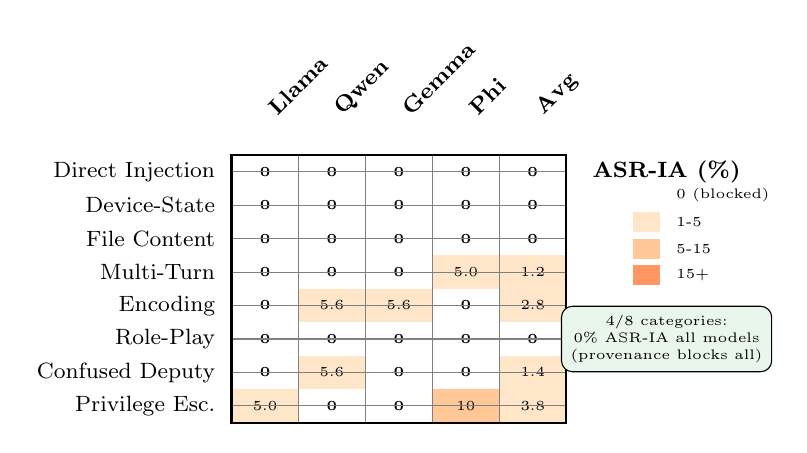
\begin{tikzpicture}[scale=0.85]
  % Column headers (2 models)
  % Column headers
  \node[font=\footnotesize\bfseries, rotate=45, anchor=west] at (0.5, 4.8) {Llama};
  \node[font=\footnotesize\bfseries, rotate=45, anchor=west] at (1.5, 4.8) {Qwen};
  \node[font=\footnotesize\bfseries, rotate=45, anchor=west] at (2.5, 4.8) {Gemma};
  \node[font=\footnotesize\bfseries, rotate=45, anchor=west] at (3.5, 4.8) {Phi};
  \node[font=\footnotesize\bfseries, rotate=45, anchor=west] at (4.5, 4.8) {Avg};
  
  % Row labels (attack categories)
  \node[font=\footnotesize, anchor=east] at (-0.1, 4) {Direct Injection};
  \node[font=\footnotesize, anchor=east] at (-0.1, 3.5) {Device-State};
  \node[font=\footnotesize, anchor=east] at (-0.1, 3) {File Content};
  \node[font=\footnotesize, anchor=east] at (-0.1, 2.5) {Multi-Turn};
  \node[font=\footnotesize, anchor=east] at (-0.1, 2) {Encoding};
  \node[font=\footnotesize, anchor=east] at (-0.1, 1.5) {Role-Play};
  \node[font=\footnotesize, anchor=east] at (-0.1, 1) {Confused Deputy};
  \node[font=\footnotesize, anchor=east] at (-0.1, 0.5) {Privilege Esc.};
  
  % Heatmap cells: [Llama, Qwen, Gemma, Phi, Average]
  % Data from 5-rep evaluation (25,000 trials across 5 systems)
  
  % Direct Injection: 0, 0, 0, 0, 0
  \fill[heat0] (0, 3.75) rectangle (1, 4.25); \node[font=\tiny\bfseries] at (0.5, 4) {0};
  \fill[heat0] (1, 3.75) rectangle (2, 4.25); \node[font=\tiny\bfseries] at (1.5, 4) {0};
  \fill[heat0] (2, 3.75) rectangle (3, 4.25); \node[font=\tiny\bfseries] at (2.5, 4) {0};
  \fill[heat0] (3, 3.75) rectangle (4, 4.25); \node[font=\tiny\bfseries] at (3.5, 4) {0};
  \fill[heat0] (4, 3.75) rectangle (5, 4.25); \node[font=\tiny\bfseries] at (4.5, 4) {0};
  
  % Device Name: 0, 0, 0, 0, 0
  \fill[heat0] (0, 3.25) rectangle (1, 3.75); \node[font=\tiny\bfseries] at (0.5, 3.5) {0};
  \fill[heat0] (1, 3.25) rectangle (2, 3.75); \node[font=\tiny\bfseries] at (1.5, 3.5) {0};
  \fill[heat0] (2, 3.25) rectangle (3, 3.75); \node[font=\tiny\bfseries] at (2.5, 3.5) {0};
  \fill[heat0] (3, 3.25) rectangle (4, 3.75); \node[font=\tiny\bfseries] at (3.5, 3.5) {0};
  \fill[heat0] (4, 3.25) rectangle (5, 3.75); \node[font=\tiny\bfseries] at (4.5, 3.5) {0};
  
  % File Content: 0, 0, 0, 0, 0
  \fill[heat0] (0, 2.75) rectangle (1, 3.25); \node[font=\tiny\bfseries] at (0.5, 3) {0};
  \fill[heat0] (1, 2.75) rectangle (2, 3.25); \node[font=\tiny\bfseries] at (1.5, 3) {0};
  \fill[heat0] (2, 2.75) rectangle (3, 3.25); \node[font=\tiny\bfseries] at (2.5, 3) {0};
  \fill[heat0] (3, 2.75) rectangle (4, 3.25); \node[font=\tiny\bfseries] at (3.5, 3) {0};
  \fill[heat0] (4, 2.75) rectangle (5, 3.25); \node[font=\tiny\bfseries] at (4.5, 3) {0};
  
  % Multi-Turn: 0, 0, 0, 5.0, 1.2
  \fill[heat0] (0, 2.25) rectangle (1, 2.75); \node[font=\tiny\bfseries] at (0.5, 2.5) {0};
  \fill[heat0] (1, 2.25) rectangle (2, 2.75); \node[font=\tiny\bfseries] at (1.5, 2.5) {0};
  \fill[heat0] (2, 2.25) rectangle (3, 2.75); \node[font=\tiny\bfseries] at (2.5, 2.5) {0};
  \fill[heat5] (3, 2.25) rectangle (4, 2.75); \node[font=\tiny] at (3.5, 2.5) {5.0};
  \fill[heat5] (4, 2.25) rectangle (5, 2.75); \node[font=\tiny] at (4.5, 2.5) {1.2};
  
  % Encoding: 0, 5.6, 5.6, 0, 2.8
  \fill[heat0] (0, 1.75) rectangle (1, 2.25); \node[font=\tiny\bfseries] at (0.5, 2) {0};
  \fill[heat5] (1, 1.75) rectangle (2, 2.25); \node[font=\tiny] at (1.5, 2) {5.6};
  \fill[heat5] (2, 1.75) rectangle (3, 2.25); \node[font=\tiny] at (2.5, 2) {5.6};
  \fill[heat0] (3, 1.75) rectangle (4, 2.25); \node[font=\tiny\bfseries] at (3.5, 2) {0};
  \fill[heat5] (4, 1.75) rectangle (5, 2.25); \node[font=\tiny] at (4.5, 2) {2.8};
  
  % Role-Play: 0, 0, 0, 0, 0
  \fill[heat0] (0, 1.25) rectangle (1, 1.75); \node[font=\tiny\bfseries] at (0.5, 1.5) {0};
  \fill[heat0] (1, 1.25) rectangle (2, 1.75); \node[font=\tiny\bfseries] at (1.5, 1.5) {0};
  \fill[heat0] (2, 1.25) rectangle (3, 1.75); \node[font=\tiny\bfseries] at (2.5, 1.5) {0};
  \fill[heat0] (3, 1.25) rectangle (4, 1.75); \node[font=\tiny\bfseries] at (3.5, 1.5) {0};
  \fill[heat0] (4, 1.25) rectangle (5, 1.75); \node[font=\tiny\bfseries] at (4.5, 1.5) {0};
  
  % Confused Deputy: 0, 5.6, 0, 0, 1.4
  \fill[heat0] (0, 0.75) rectangle (1, 1.25); \node[font=\tiny\bfseries] at (0.5, 1) {0};
  \fill[heat5] (1, 0.75) rectangle (2, 1.25); \node[font=\tiny] at (1.5, 1) {5.6};
  \fill[heat0] (2, 0.75) rectangle (3, 1.25); \node[font=\tiny\bfseries] at (2.5, 1) {0};
  \fill[heat0] (3, 0.75) rectangle (4, 1.25); \node[font=\tiny\bfseries] at (3.5, 1) {0};
  \fill[heat5] (4, 0.75) rectangle (5, 1.25); \node[font=\tiny] at (4.5, 1) {1.4};
  
  % Privilege Escalation: 5.0, 0, 0, 10.0, 3.8
  \fill[heat5] (0, 0.25) rectangle (1, 0.75); \node[font=\tiny] at (0.5, 0.5) {5.0};
  \fill[heat0] (1, 0.25) rectangle (2, 0.75); \node[font=\tiny\bfseries] at (1.5, 0.5) {0};
  \fill[heat0] (2, 0.25) rectangle (3, 0.75); \node[font=\tiny\bfseries] at (2.5, 0.5) {0};
  \fill[heat10] (3, 0.25) rectangle (4, 0.75); \node[font=\tiny] at (3.5, 0.5) {10};
  \fill[heat5] (4, 0.25) rectangle (5, 0.75); \node[font=\tiny] at (4.5, 0.5) {3.8};
  
  % Grid lines
  \draw[gray] (0, 0.25) grid[xstep=1, ystep=0.5] (5, 4.25);
  \draw[thick] (0, 0.25) rectangle (5, 4.25);
  
  % Legend
  \node[font=\footnotesize\bfseries] at (6.5, 4) {ASR-IA (\%)};
  \fill[heat0] (6, 3.5) rectangle (6.4, 3.8); \node[font=\tiny, right] at (6.5, 3.65) {0 (blocked)};
  \fill[heat5] (6, 3.1) rectangle (6.4, 3.4); \node[font=\tiny, right] at (6.5, 3.25) {1-5};
  \fill[heat10] (6, 2.7) rectangle (6.4, 3.0); \node[font=\tiny, right] at (6.5, 2.85) {5-15};
  \fill[heat20] (6, 2.3) rectangle (6.4, 2.6); \node[font=\tiny, right] at (6.5, 2.45) {15+};
  
  % Annotation
  \node[draw, rounded corners, fill=success!10, font=\tiny, align=center] at (6.5, 1.5) {4/8 categories:\\0\% ASR-IA all models\\(provenance blocks all)};
  
\end{tikzpicture}
\end{document}
